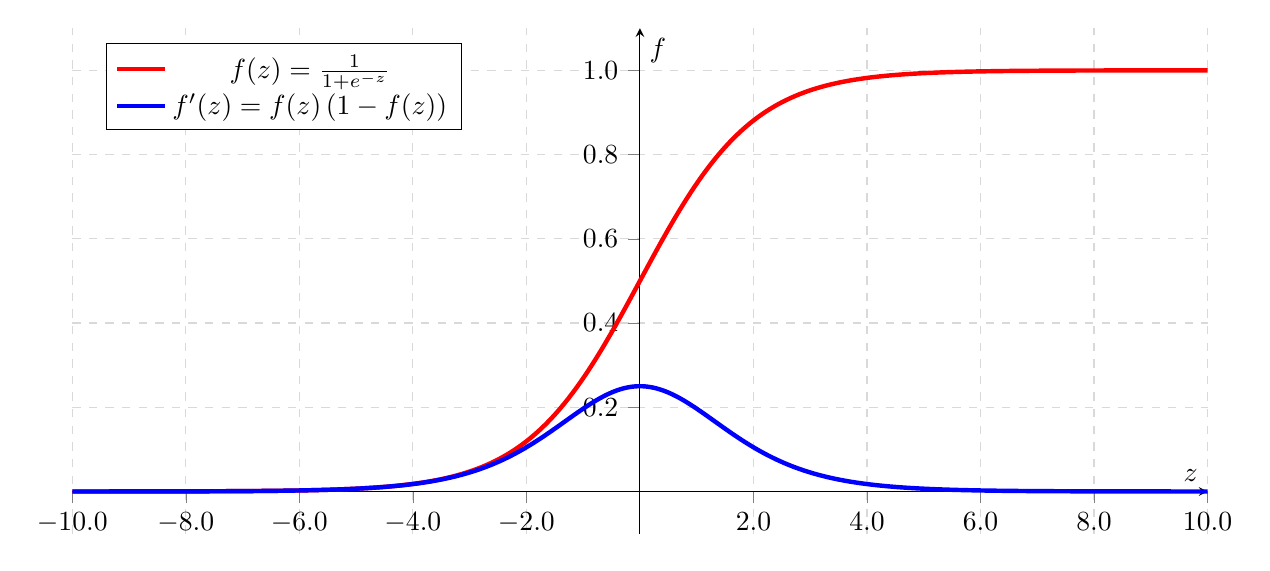
\begin{tikzpicture}
    \begin{axis}[
    	legend pos=north west,
        axis x line=middle,
        axis y line=middle,
        x tick label style={/pgf/number format/fixed,
                            /pgf/number format/fixed zerofill,
                            /pgf/number format/precision=1},
        y tick label style={/pgf/number format/fixed,
                            /pgf/number format/fixed zerofill,
                            /pgf/number format/precision=1},
        grid = major,
        width=16cm,
        height=8cm,
        grid style={dashed, gray!30},
        xmin=-10,     % start the diagram at this x-coordinate
        xmax= 10,    % end   the diagram at this x-coordinate
        ymin= -0.1,     % start the diagram at this y-coordinate
        ymax= 1.1,   % end   the diagram at this y-coordinate
        %axis background/.style={fill=white},
        xlabel=$z$,
        ylabel=$f$,
        tick align=outside,
        enlargelimits=false]
      % plot the stirling-formulae
      \addplot[domain=-10:10, red, ultra thick,samples=500] {1/(1+exp(-x))};
      \addplot[domain=-10:10, blue, ultra thick,samples=500] {exp(-x)/((1+exp(-x))*(1+exp(-x)))};
      \addlegendentry{$f(z)=\frac{1}{1+e^{-z}}$}
      \addlegendentry{$f^{\prime}(z)=f(z)\left(1-f(z)\right)$}
    \end{axis}
\end{tikzpicture}